\documentclass[11pt, a4paper]{article}




\usepackage[utf8]{inputenc}		% Zeichen in UTF-8 speichern (?)
\usepackage[T1]{fontenc}		% Sonderzeichen richtig darstellen
\usepackage[british]{babel}		% versch. Sonderzeichen, Silbentrennung, Gliederung
\usepackage[margin=25mm, top=38mm, bottom=20mm, headheight=40pt]{geometry}
\usepackage{fancyhdr}			% Kopf- und Fußnoten
\usepackage{multicol}			% mehrere Spalten
\usepackage{lastpage}			% Seite x von y
\usepackage{tabularx}    		% Tables of specified width
\usepackage{graphicx}			% Einstellmöglichkeiten für Bilder
\usepackage{caption}			% Einstellmöglichkeiten Tabellen- und Bildunterschriften, captionof
\usepackage{array}
\usepackage{booktabs}
\usepackage{siunitx}			% SI-Einheiten
\usepackage{mathtools}			% macht die Matheumgebung, Weiterentwicklung von amsmath
\usepackage{amssymb}			% Erweiterung des Zeichensatzes, beinhaltet amsfonts
\usepackage{verbatim}			% macht die "comment-Umgebung"
\usepackage[hidelinks]{hyperref}
\usepackage{setspace}
\usepackage{epstopdf}




%\addto{\captionsbritish}{
%\renewcommand{\figurename}{Fig.}
%\renewcommand{\tablename}{Tab.}
%}


\setlength{\parindent}{0pt}

\setlength{\columnsep}{8mm}

\clubpenalty10000
\widowpenalty10000
\displaywidowpenalty = 10000


\pagestyle{fancy}
\fancyhf{}
\lhead{something}
\rhead{Page \thepage\ of \pageref{LastPage}}


% new column types for tabularx
\newcolumntype{Y}{>{\raggedright\arraybackslash}X} % X column left aligned
\newcolumntype{W}{>{\raggedleft\arraybackslash}X}  % X column right aligned
\newcolumntype{Z}{>{\centering\arraybackslash}X}   % X column centered


\newenvironment{Figure}
  {\par\medskip\noindent\minipage{\linewidth}}
  {\endminipage\par\medskip}
\renewcommand{\arraystretch}{1.2}


\sisetup{per-mode = symbol}
















\begin{document}

\begin{titlepage}
	
	%institut logoer findes her:
	%http://portalen.dtu.dk/DTU_Generelt/APK/Services/Kommunikation/Designguide.aspx
	
	\begin{minipage}{0.5\textwidth}
		\begin{flushleft}
			%\textbf{Group ??} \\
			%
			\textbf{\today} \\
			\vspace{0.1cm} 
			Maike Fröhner - s172033 \\
			Naya Sophie Rye Jørgensen - s173087 \\
			Vaidehi Narsingh - s171883 \\
			\vspace{0.1cm}
			Supervisor: Leif Toudal Pedersen
			
			
			
		\end{flushleft}
	\end{minipage}
	\hfill
	\begin{minipage}{0.1\textwidth}
		\begin{flushright}
			
\includegraphics[width=1\textwidth]{DTU_logo1.png}
		\end{flushright}
	\end{minipage}\\	% ***
	
	
	\begin{center}
		\vspace*{\stretch{1}}
		\rule{\textwidth}{1mm}\\
		%\vspace{0.25cm}
		% ***
		\Huge\bfseries Retrieval of Atmospheric and Oceanic Parameters from AMSR Satellite Data\\ 				% ***
		%\vspace{1cm}
		\rule{\textwidth}{1mm}\\
		\vspace{0.5cm}
		%\Large Mandatory Assignment\\[0.3cm]
		\Large 30350 Remote Sensing \\[0.5cm]
		\vspace*{\stretch{1}}
		%\begin{figure}[h]
		%
		%%\centering
		%%\includegraphics[width=0.5\textwidth]{fig/pca}
		%%\label{fig:big_brother}
		%\end{figure}						% ***			 
		
		
		
		\vspace{0.5cm}
		\vspace*{\stretch{2}}
	\end{center}
	
	\begin{minipage}{0.3\textwidth}
		\begin{flushleft}
			
\includegraphics[height=1.2cm]{DTU-Space.png} 	% ***
	\end{flushleft}\end{minipage}
\end{titlepage}

\pagestyle{fancy}
\fancyhf{} 
\fancyhead[LE,RO]{ \thepage}
\fancyhead[LO]{Retrieval of Atmospheric and Oceanic Parameters from AMSR Satellite Data}

%\tableofcontents
%\addtocontents{toc}{\setcounter{tocdepth}{2}}



















\newpage
\section{Introduction}

The purpose of the project is to develop and apply a model that retrieves geophysical parameters from brightness temperature measured by the radiometer onboard the AMSR satellite. Atmospheric and oceanic parameters can be obtained in a variety of ways, ranging from in-situ observations through satellite observations using microwave techniques to numerical weather models including analysis and forecasts.

\begin{figure}[h]
   \centering
   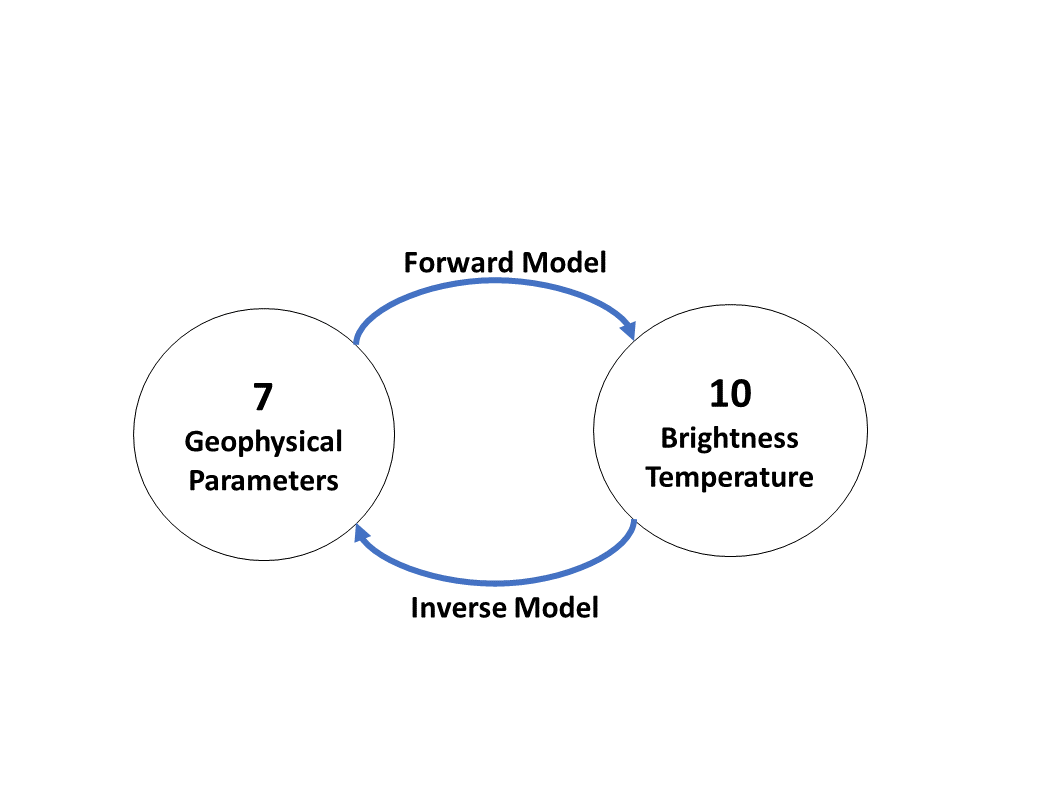
\includegraphics[width=0.6\textwidth]{Flowchart.png}
   \caption{Naya. please write a caption}
   \label{fig:flow}
\end{figure}

An existing climatological model computing the brightness temperatures measured by the radiometer from the geophysical parameters Wind Speed, Water Vapour, Cloud Liquid Water, Sea Surface Temperature, Ice Surface Temperature, Sea Ice Concentration and Multi-year Ice Fraction shall be validatet in the course of this project. We will then use this forward model to develop an inverse model, which will be applied to study geophysical parameters from globally measured brightness temperatures.
\newline

\begin{comment}
 (from climatological weather prediction by ESA) computing the Brightness Temperature for 10 AMSR channels (6, 10, 18, 23, 36 GHz H and V polarisation). Furthermore, Using Inverse model, we retrieved the geophysical parameters important for analysing and studying the global hydrological cycle and radiative balance. (from the measured brightness temperature).
Project describes the forward model is expanded to develop Inverse Model. Furthermore, it includes a section on how the forward and Inverse model has been verified and a section with some real-time application of the use of Inverse algorithm. 
However, the results presented shows that algorithm is too sensitive to geophysical noise. It is therefore vital to include a priori knowledge of these geophysical parameters in the retrieval process, which has been taken care in our project.
\end{comment}

The structure of this document is as follows: First, the forward model will be introduced and validated. Then the inverse model will be developed, configured and validated. Then the influence of different radiometric channels and different geophysical parameters is studied. Finally, we conclude with the summary of results obtained by the examples and discussion of results.
















\newpage
\section{Validation of the Forward Model}

The forward model computes from a set of oceanic and atmospheric parameters the brightness temperatures expected to be measured by a satellite radiometer. The input parameters are listed in Table \ref{tab:input_parameters}, and the output parameters include values for both horizontal and vertical polarization at \SI{6.93}{GHz}, \SI{10.65}{GHz}, \SI{18.70}{GHz}, \SI{23.80}{GHz}, and \SI{36.50}{GHz}.

\begin{table}[h!]
\centering
\begin{tabular}{@{}p{4cm} p{1.8cm}p{2.8cm}p{1.8cm}p{1.8cm}@{}}
\tabularnewline
& \multicolumn{2}{c}{Forward Model} & \multicolumn{2}{c}{Reference Data}
\tabularnewline
\cmidrule(r{1em}){2-3} \cmidrule(l{1em}){4-5}
& Abbrev. & Unit & Abbrev. & Unit
\tabularnewline
\midrule
Ice concentration	& C\_is	& fraction		& ci	& fraction	\\
MY-fraction		& F\_MY	& fraction		& 	& 		\\
Ice temperature		& T\_is	& \SI{}{K}	& skt	& \SI{}{K}	\\
Water vapour		& V	& \SI{}{mm} (columnar)	& tcwv	& \SI{}{kg/m^2}	\\
Cloud liquid water	& L	& \SI{}{mm} (columnar)	& tclw	& \SI{}{kg/m^2}	\\
Wind speed		& W	& \SI{}{m/s}		& ws	& m/s		\\
Sea surface temperature	& T\_ow	& \SI{}{K}	& sst	& \SI{}{K}	\\
\midrule
\end{tabular}
\caption{Atmospheric and oceanic parameters entered into the forward model}
\label{tab:input_parameters}
\end{table}

This forward model was validated by comparing its results to reference data from ESA's ``Sea Ice Climate Change Initiative''.


\subsection{Description of the Reference Data}

The reference data consists of brightness temperatures at the relevant polarizations and frequencies as measured by the AMSR2 radiometer onboard the GCOM-W1 satellite. The measured data is paired with validated sea ice concentrations and numerical weather predictions for the atmospheric and oceanic parameters at the same geocoded locations at near simultaneous time. There are two different data sets: one with an ice concentration of 0, the other one with an ice concentration of 1. The data points of each set cover the entire year 2014. The dataset with the no ice condition covers latitudes between 5 and 73 degrees, and the dataset with an ice concentration of 1 covers latitudes between 78.5 and 87.5 degrees. A description of the dataset can be found in \cite{Wink2}.

\subsubsection{Potential Sources of Errors}
\label{sec:RefDat}
When using this reference data package to validate the forward model, several points have to be taken into account: Firstly, the forward model was developed for the AMSR-E instrument. To use the atmospheric and oceanic parameters as input in the forward model in order to compare the output with the AMSR2 measured brightness temperatures, we applied a conversion to these brightness temperatures as suggested in \cite{secret}. For the \SI{6.93}{GHz} channel we used the correction for \SI{7}{GHz} throughout the document.
%The AMSR-E instrument on the NASA satellite EOS Aqua was operational between May 4, 2002 and October 4, 2011, and the AMSR2 instrument mounted on the JAXA satellite GCOM-W1, has been in operation since May 18, 2012. 
\newline

Secondly, the reference data does not contain information about the multi-year ice fraction needed as input in the forward model. For the data set with an ice concentration of 0, the MY fraction is irrelevant. It is therefore possible to validate the forward model for the open water datapoints. For the data set with an ice concentration of 1, a multi-year ice concentration of 0.5 was assumed. This dataset can therefore be used as a coherency check, but not to validate the model.
\newline

Thirdly, as mentioned above, the geophysical parameters given in the reference data were computed from numerical weather predictions, and their uncertainty is not known. In particular, this is also not discussed in \cite{Wink2}. We suspect the error on the cloud liquid water to be especially large. This parameter is increasingly influential towards higher frequency channels, were an error in the prediction would accordingly cause a larger error in the brightness temperatures.

\subsubsection{Practical Considerations}
The wind speed is given in the reference data as a u-component, v-component, and as a composite of the two. %(comment/question: where u and v denote zonal and meridional directions respectively?)
We chose to use the composite value for the wind speed as the input in the forward model. %(Argumentation!?) (-backscatter as a result of wind speed direction (upwind, downwind, crosswind) sensitive to azimuth angle \cite{Elachi})
The parameters ``water vapour'' and ``cloud liquid water'', which are given in the columnar units of $\SI{}{kg/m^2}$ in the reference data, were converted to $\SI{}{mm}$, indicating the height of water vapor or cloud liquid water if condensed uniformly across the column. $\SI{1}{kg/m^2}$ corresponds to $\SI{1}{mm}$ \cite{remss}.


\subsection{Validation Procedure}

For the data set with an ice concentration of 0, the atmospheric and oceanic parameters were entered into the forward model, and the difference between the modelled brightness temperatures and the corrected brightness temperatures from the reference data was recorded:
\[
e=T_\text{B, modelled} - T_\text{B, reference, corrected}
\]
The reference file has 6988 data points, every second of which was used. For the data set with an ice concentration of 1, the atmospheric and oceanic parameters were entered together with guessed values for the multi-year ice fraction of 0, 0.5, and 1, consecutively. The multi-year ice fraction was chosen to be constant for all datapoints to simplify the validation process. Of the 10936 reference data points recorded between October and May, every second point was used.


\subsection{Validation Results}
\label{sec:ForValRes}

The discrepancies for the no ice condition are shown in Table \ref{tab:for0}, and those for the ice condition are shown in Tables \ref{tab:for1_0} to \ref{tab:for1_1}.

\begin{table}[h!]
\centering
\begin{tabular}{@{} l l l l l l l @{}}
Channel & 6.93v & 6.93h & 10.65v & 10.65h & 18.70v & 18.70h \\
\midrule
Mean & \SI{0.1027}{K} & \SI{-0.2817}{K} & \SI{-1.1832}{K} & \SI{-2.8420}{K} & \SI{3.7785}{K} & \SI{1.8898}{K} \\
Std. Dev. & \SI{1.4176}{K} & \SI{2.9155}{K} & \SI{2.1227}{K} & \SI{3.7947}{K} & \SI{10.2530}{K} & \SI{12.9650}{K} \\
\midrule
\tabularnewline
\end{tabular}
\begin{tabular}{@{} l l l l l @{}}
Channel & 23.80v & 23.80h & 36.50v & 36.50h \\
\midrule
Mean & \SI{-1.5822}{K} & \SI{-4.7026}{K} & \SI{-2.2742}{K} & \SI{-5.8099}{K} \\
Std. Dev. & \SI{3.6383}{K} & \SI{7.1321}{K} & \SI{4.6630}{K} & \SI{10.2386}{K} \\
\midrule
\end{tabular}
\caption{Modelled brigthness temperatures compared to the corrected no-ice dataset}
\label{tab:for0}
\end{table}

In addition, histograms were plotted for the error distribution of the no ice condition (only for the channels with the most notable offset), as well as of the ice condition for a multi-year ice concentration of 0.5 (all channels). These are shown in Figures \ref{fig:for0dist} and \ref{fig:for1dist}. The occurence rate is normalized to the number of data points. It can be observed, that the channels for \SI{10.65}{GHz} and higher frequencies have double peaks, which could correspond to the points of no/full ice concentration in the data set. All channels have a negative bias, i.e. the modelled brightness temperatures are smaller than the ones in the reference data. \\

\begin{table}[h!]
\centering
\begin{tabular}{@{} l l l l l l l @{}}
Channel & 6.93v & 6.93h & 10.65v & 10.65h & 18.70v & 18.70h \\
\midrule
Mean & \SI{-18.8904}{K} & \SI{-36.1881}{K} & \SI{-18.8032}{K} & \SI{-30.2216}{K} & \SI{-4.7582}{K} & \SI{-11.3865}{K} \\
Std. Dev. & \SI{4.9079}{K} & \SI{7.4777}{K} & \SI{5.6295}{K} & \SI{9.6398}{K} & \SI{11.0927}{K} & \SI{14.1847}{K} \\
\midrule
\tabularnewline
\end{tabular}
\begin{tabular}{@{} l l l l l @{}}
Channel & 23.80v & 23.80h & 36.50v & 36.50h \\
\midrule
Mean & \SI{1.3569}{K} & \SI{-1.4115}{K} & \SI{9.5846}{K} & \SI{9.5860}{K} \\
Std. Dev. & \SI{14.3928}{K} & \SI{16.7768}{K} & \SI{19.4340}{K} & \SI{20.2949}{K} \\
\midrule
\end{tabular}
\caption{Modelled brigthness temperatures compared to the corrected dataset with an ice concentration of 1, multi-year ice fraction 0}
\label{tab:for1_0}
\end{table}



\begin{table}[h!]
\centering
\begin{tabular}{@{} l l l l l l l @{}}
Channel & 6.93v & 6.93h & 10.65v & 10.65h & 18.70v & 18.70h \\
\midrule
Mean & \SI{-13.0277}{K} & \SI{-22.3905}{K} & \SI{-16.9252}{K} & \SI{-22.8343}{K} & \SI{-10.8922}{K} & \SI{-15.9716}{K} \\
Std. Dev. & \SI{5.0466}{K} & \SI{7.5811}{K} & \SI{5.6564}{K} & \SI{9.6501}{K} & \SI{11.0802}{K} & \SI{14.1971}{K} \\
\midrule
\tabularnewline
\end{tabular}
\begin{tabular}{@{} l l l l l @{}}
Channel & 23.80v & 23.80h & 36.50v & 36.50h \\
\midrule
Mean & \SI{-7.9716}{K} & \SI{-8.9957}{K} & \SI{-6.1945}{K} & \SI{-4.2009}{K} \\
Std. Dev. & \SI{14.4112}{K} & \SI{16.8180}{K} & \SI{19.4457}{K} & \SI{20.3167}{K} \\
\midrule
\end{tabular}
\caption{Modelled brigthness temperatures compared to the corrected dataset with an ice concentration of 1, multi-year ice fraction 0.5}
\label{tab:for1_5}
\end{table}



\begin{table}[h!]
\centering
\begin{tabular}{@{} l l l l l l l @{}}
Channel & 6.93v & 6.93h & 10.65v & 10.65h & 18.70v & 18.70h \\
\midrule
Mean & \SI{-7.1651}{K} & \SI{-8.5928}{K} & \SI{-15.0473}{K} & \SI{-15.4471}{K} & \SI{-17.0261}{K} & \SI{-20.5568}{K} \\
Std. Dev. & \SI{5.1993}{K} & \SI{7.7493}{K} & \SI{5.6848}{K} & \SI{9.6754}{K} & \SI{11.0758}{K} & \SI{14.2130}{K} \\
\midrule
\tabularnewline
\end{tabular}
\begin{tabular}{@{} l l l l l @{}}
Channel & 23.80v & 23.80h & 36.50v & 36.50h \\
\midrule
Mean & \SI{-17.3001}{K} & \SI{-16.5760}{K} & \SI{-21.9737}{K} & \SI{-17.9878}{K} \\
Std. Dev. & \SI{14.4461}{K} & \SI{16.8686}{K} & \SI{19.4906}{K} & \SI{20.3633}{K}  \\
\midrule
\end{tabular}
\caption{Modelled brigthness temperatures compared to the corrected dataset with an ice concentration of 1, multi-year ice fraction 1}
\label{tab:for1_1}
\end{table}


\begin{figure}[h!]
   \centering
   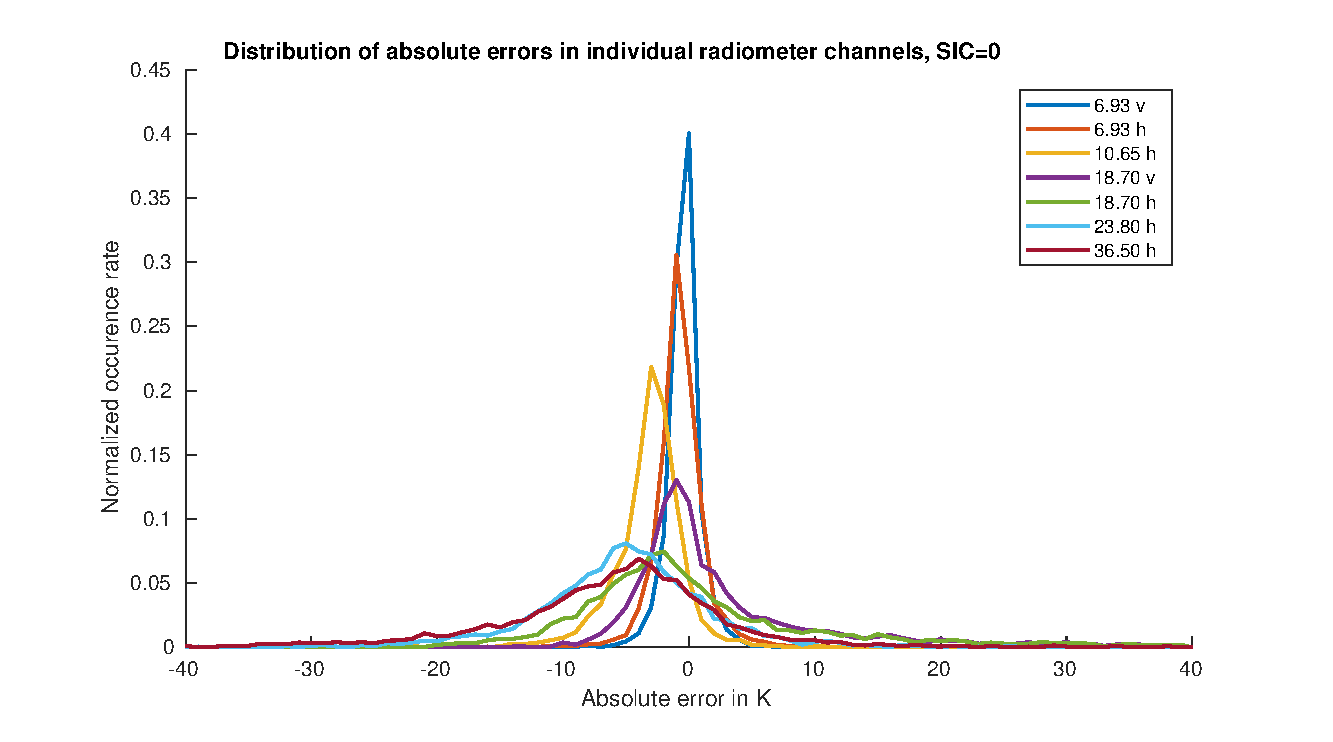
\includegraphics[width=0.9\textwidth]{ValidationForward_SIC0_errordist.eps}
   \caption{Distribution of the errors of the modelled brightness temperatures compared to the no ice dataset; only some channels are shown}
   \label{fig:for0dist}
\end{figure}

\begin{figure}[h!]
   \centering
   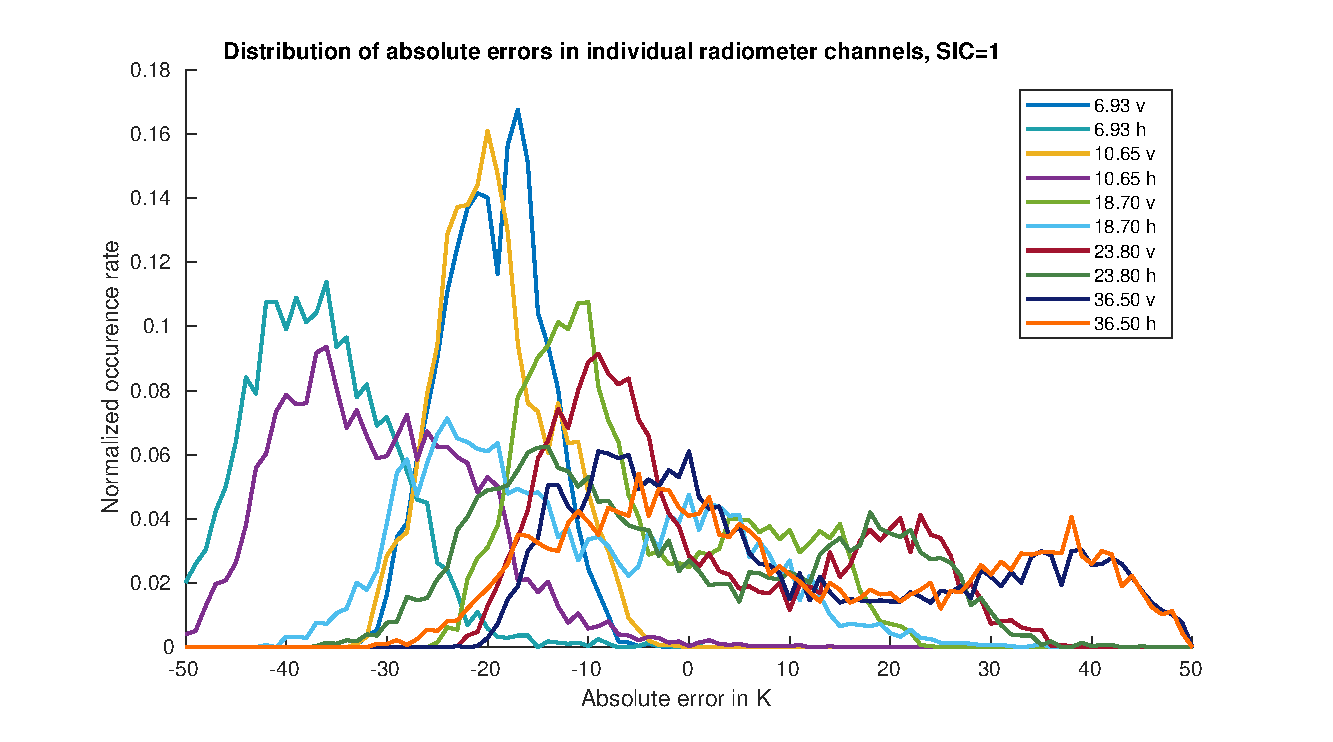
\includegraphics[width=0.9\textwidth]{ValidationForward_SIC1_errordist.eps}
   \caption{Distribution of the errors of the modelled brightness temperatures compared to the no ice dataset; multi-year ice concentration 0.5}
   \label{fig:for1dist}
\end{figure}



The forward model is not under all conditions able to reproduce the brightness temperatures expected from the reference data. We do not know, which of the contributions listed in \mbox{section \ref{sec:RefDat}} causes the errors. To further investigate this problem is beyond the scope of this project, and we will therefore limit our use of the model to no ice cases for the following tasks.











\clearpage
\section{Development of the Inverse Model}

To compute the oceanic and atmospheric parameters from the set of brightness temperatures measured by the satellite radiometer, an inverse model was developed using estimation theory. The inverse model essentially employs the forward model to compute an estimate of the brightness temperatures from an estimate of the geophysical parameters, then compares the estimated brightness temperatures to the measured brightness temperatures, and finally improves the estimate for the geophysical parameters based on the result of the comparison (see figure \ref{fig:block} for a graphical representation). Once the estimated brightness temperatures come close enough to the measured ones, the geophysical parameters last inputted are considered a good estimate and delivered as the result of the inverse modelling. This is explained in more detail in the next subsection.
\newline

The inverse model was then validated by comparing it to the forward model. It was not compared to any external data source.


\subsection{Algorithm of the Inverse Model}

The input of the inverse model function is a 10 element vector \(T_\text{B,m}\) containing the brightness temperatures measured for each of the radiometer channels.
\newline

\begin{figure}[h]
   \centering
   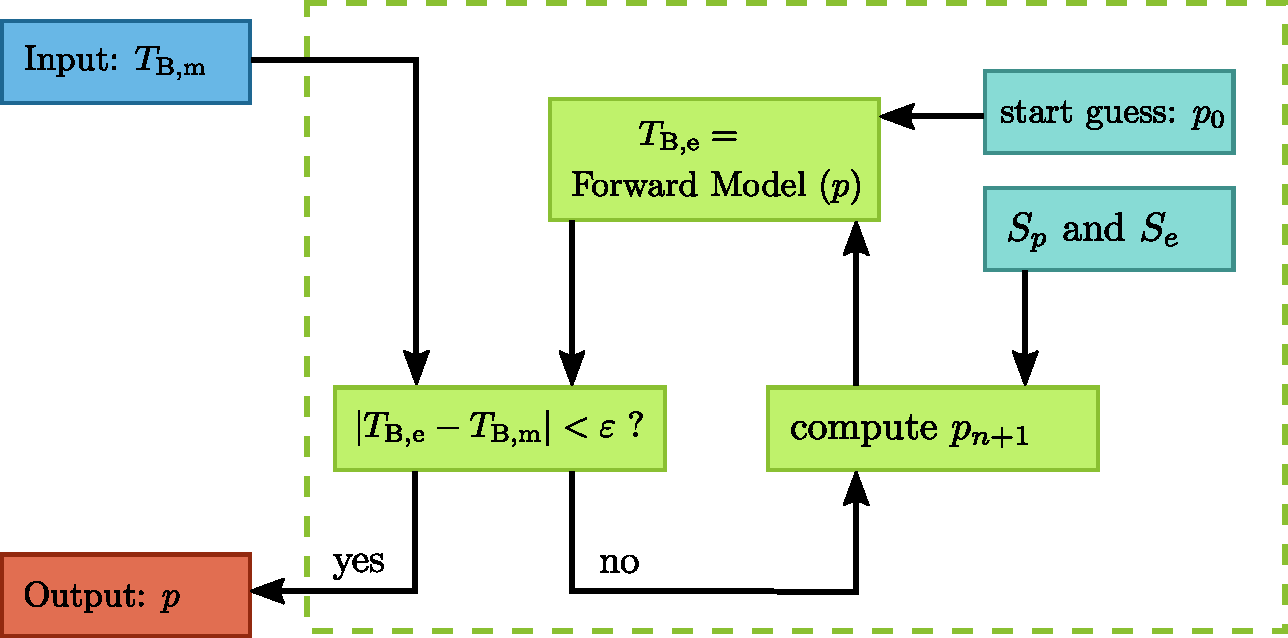
\includegraphics[width=0.6\textwidth]{blockdiagramm.pdf}
   \caption{Blockdiagramm of the inverse model function}
   \label{fig:block}
\end{figure}


The inverse model enters a 7 element vector \(p\) containing estimates of the geophysical parameters listed in table \ref{tab:input_parameters} into the forward model and retrieves a 10 element vector \(T_\text{B,e}\) containing estimated brightness temperatures for each channel. In the first iteration, \(p\) is a generic guess, which is hard coded into the inverse model function. The estimated brightness temperatures \(T_\text{B,e}\) are then compared to the measured brightness temperatures \(T_\text{B,m}\).
\newline

If the estimated and the measured brightness temperatures do not agree within a range of \(\varepsilon\), a vector \(p_{n+1}\) for the (n+1)\textsuperscript{th} iteration is computed from the vector \(p_n\) of the current iteration as follows:

\begin{equation*}
p_{n+1} =
p_n   +   \Big(S_p^{-1} + M_n^T S_e^{-1} M_n \Big)^{-1}   \cdot   \Big(M_n^T S_e^{-1} (T_\text{B,m} - T_\text{B,e,n}) + S_p^{-1} (p_0 - p_n) \Big)
\end{equation*}

\ \\
Herein, \(S_p\) is the 7 by 7 covariance matrix of the geophysical parameters indicating the uncertainty attached to the start guess. Small values on the diagonal of this matrix correspond to a high confidence in the start guess and cause \(p_{n+1}\) to be close to \(p_0\). \(S_e\) is the 10 by 10 covariance matrix of the brightness temperatures measured by the radiometer. Small values on the diagonal of this matrix correspond to a high confidence into the accuracy of the radiometer, and much weight is assigned to the difference between the estimated and measured brightness temperatures, accordingly.
\newline

\(M_n\) is a 7 by 10 matrix, and it contains the partial derivatives of the brightness temperatures with respect to the geophysical parameters. This matrix is computed for every iteration. To find the element in the i\textsuperscript{th} line and j\textsuperscript{th} column of \(M\), the i\textsuperscript{th} geophysical parameter is perturbed slightly, the forward model is called for the altered vector p, and the resulting perturbation of the brightness temperature in the j\textsuperscript{th} channel is recorded. The partial derivative is then obtained by dividing the brightness temperature perturbation by the perturbation of the geophysical parameter. Large values in \(M\) correspond to a high sensitivity of the radiometer to changes in the geophysical parameters.
\newline

The partial derivatives are only valid for those values of \(p\) at which they were computed - i.e. those of the past iteration. The inverse model extrapolates these derivatives to find \(p_{n+1}\) for the next iteration. If the relations of the geophysical parameters and the brightness temperatures were entirely linear, this extrapolation would be entirely accurate and only one iteration would be needed to find the suitable vector \(p\). The less linear the system is, the less accurate is the extrapolation, and the more iterations are needed.
\newline

If the estimated and the measured brightness temperatures do agree within a range of \(\varepsilon\), the current vector p is outputted as a sufficiently accurate estimation of the geophysical parameters.


\subsection{Choice of Model Parameters}

Suitable values for the start guess of the atmospheric and oceanic parameters (\(p_0\)) and for the covariance matrix \(S_p\) were found by computing the mean and variance of the individual parameters from the reference data sets. As the data sets cover all seasons and almost the entire globe (see section \ref{sec:RefDat}), we believe this reference to be a broad enough base for computing a generic mean and variance. The values for both are listed below; the elements being in the order wind speed, water vapour, liquid water, sea surface temperature, ice temperature, ice concentration, multiyear ice fraction. The units correspond to those given in \mbox{table \ref{tab:input_parameters}}.

\begin{equation*}
p_0 =
\begin{pmatrix}
   6.1327 & 7.7035 & 0.0295 & 273.5503 & 265.0088 & 0.5000 & 0.5000
\end{pmatrix}
\end{equation*}

\begin{equation*}
S_p =
\begin{pmatrix}
   9.2865 & 0 & 0 & 0 & 0 & 0 & 0 \\
   0 & 62.1415 & 0 & 0 & 0 & 0 & 0 \\
   0 & 0 & 0.0056 & 0 & 0 & 0 & 0 \\
   0 & 0 & 0 & 22.5386 & 0 & 0 & 0 \\
   0 & 0 & 0 & 0 & 98.6461 & 0 & 0 \\
   0 & 0 & 0 & 0 & 0 & 1 & 0 \\
   0 & 0 & 0 & 0 & 0 & 0 & 1
\end{pmatrix}
\end{equation*}

\ \\
For each of the radiometer channels, an uncertainty of \SI{0.4}{K} was assumed. This leads to \SI{0.16}{K^2} for each element of the diagonal of \(S_e\).


\subsection{Validation of Inverse Model}

The inverse model is intended to be an inversion of the forward model. This means that in comparison to any reference, the inverse model can at most be as accurate as the forward model. The inverse model was therefore validated by comparison to the forward model: 
\begin{itemize}
\item for a given set of geophysical parameters, brightness temperatures were computed by the forward model
\item these brightness temperatures were entered into the inverse model, which computed an estimate of the geophysical parameters (\(p_\text{estimated}\))
\item the estimate was then compared to the original set of geophysical parameters (\(p_\text{originial}\)), the error being described as follows:
\end{itemize}
\begin{equation*}
e = p_\text{estimated} - p_\text{original}
\end{equation*}

\ \\
The reference data sets used to validate the forward model were used as a generic source of geophysical parameters to be inputted into the forward model. They were not used as a reference to compare modelled results to! Unfortunately, the data sets contain some outliers, which cause the inverse model to not converge. We therefore restricted the number of iterations to 10 to be able to automatically run the inversion model on all data points. The results of the inverse model did not improve for a higher number of iterations. 
\newline

Using all data points of the no ice data file, the inverse model produces the error described in Table \ref{tab:errorinv}. A closer investigation revealed that the error does not arise evenly distributed over the used input data points: for high sea surface temperatures, which come together with high amounts of liquid and gaseous water in the atmosphere, the error can become very large. This is exemplarily illustrated in Figure \ref{fig:sstError}, where the input sea surface temperature (\( p_\text{original} \)) is shown together with the error on the sea surface temperature (\( e \)) produced by the inverse model.
\newline

\begin{table}[h]
\centering
\begin{tabular}{@{} l l l l l l @{}}
Parameter & ws [\SI{}{m/s}] & tcwv [\SI{}{\kilo\gram\per\square\meter}] & tclw [\SI{}{\kilo\gram\per\square\meter}] & sst [\SI{}{K}] & ci [fraction] \\
\midrule
Mean & \SI{-0.3915}{} & \SI{0.0927}{} & \SI{0.0013}{} & \SI{-1.2479}{} & \SI{0.0236}{} \\
Std. Dev. & \SI{6.4720}{} & \SI{5.5608}{} & \SI{0.0798}{} & \SI{16.6951}{} & \SI{0.4234}{} \\
\midrule
\end{tabular}
\caption{Estimated parameters compared to the original parameters}
\label{tab:errorinv}
\end{table}

When the input data is restricted to points with a sea surface temperature below \SI{283}{K}, the accuracy of the inverse model improves. This excludes 2492 data points. The remaining error is described in Table \ref{tab:errorinvrest}.
\newline

\begin{table}[h]
\centering
\begin{tabular}{@{} l l l l l l @{}}
Parameter & ws [\SI{}{m/s}] & tcwv [\SI{}{\kilo\gram\per\square\meter}] & tclw [\SI{}{\kilo\gram\per\square\meter}] & sst [\SI{}{K}] & ci [fraction] \\
\midrule
Mean & \SI{-0.5640}{} & \SI{0.0216}{} & \SI{0.0011}{} & \SI{-0.5747}{} & \SI{0.0065}{} \\
Std. Dev. & \SI{1.0443}{} & \SI{0.0499}{} & \SI{0.0066}{} & \SI{0.5919}{} & \SI{0.0131}{} \\
\midrule
\end{tabular}
\caption{Estimated parameters compared to the original parameters, with the input data restricted to points with a sea surface temperature below \SI{283}{K}}
\label{tab:errorinvrest}
\end{table}


\begin{figure}[h]
   \centering
   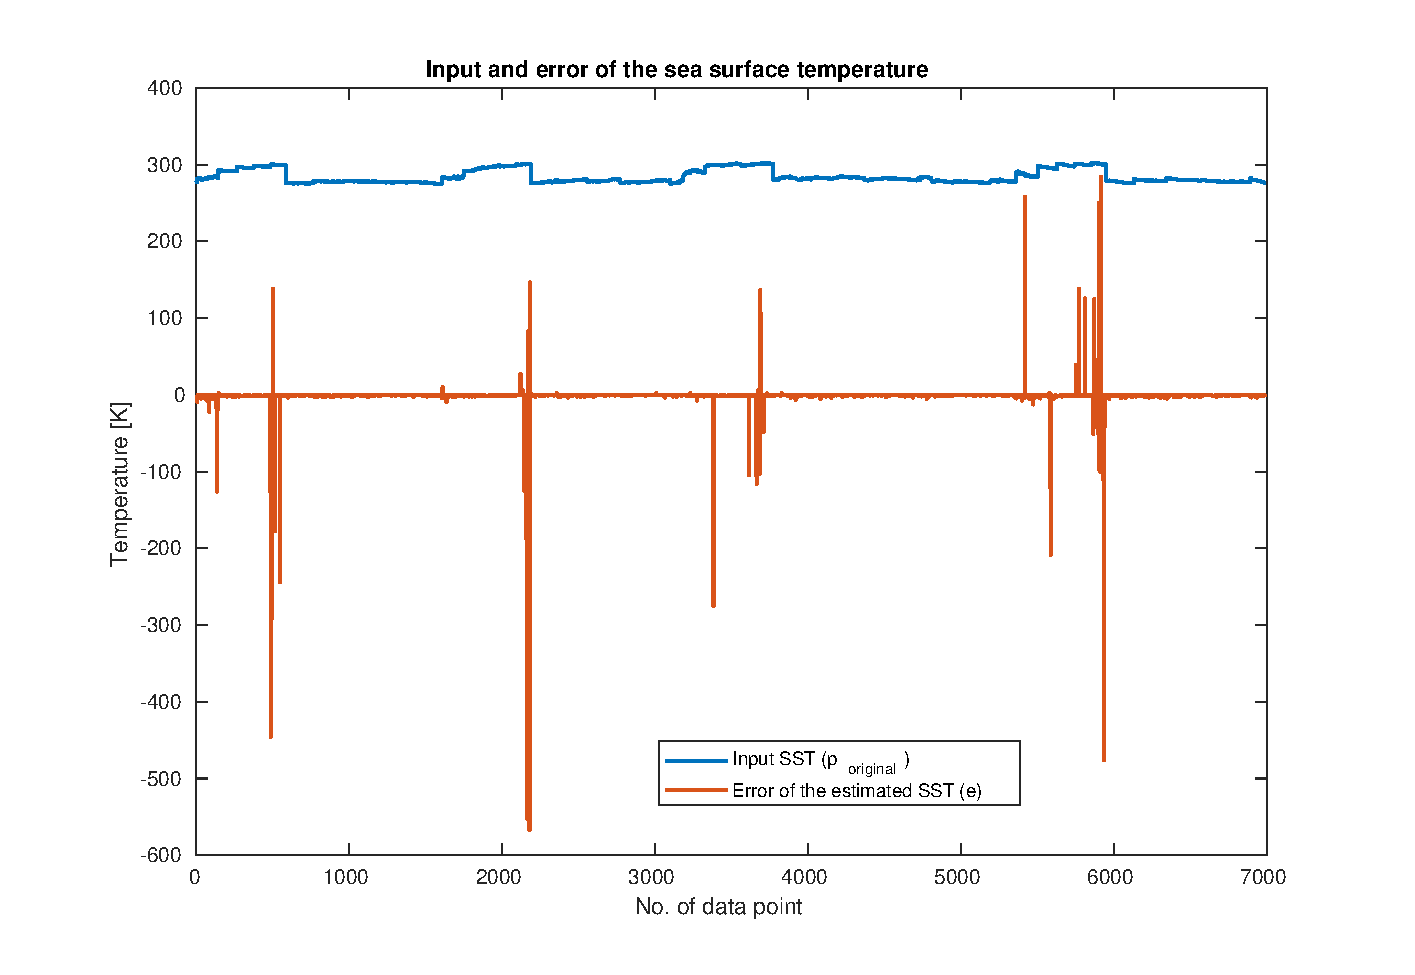
\includegraphics[width=0.9\textwidth]{ValidationInverse_SIC0_sstError.eps}
   \caption{The error of the inverse model (red) can become very large for high sea surface temperatures (blue).}
   \label{fig:sstError}
\end{figure}

We conclude that the inverse model is very sensitive to high sea surface temperatures and atmospheric water contents, but performs satisfactory otherwise.

\clearpage












\section{Application of Inverse Model}
\subsection{The Effect of Channel Selection on Sea Surface Temperature Retrieval}
The inverse model is applied to the AMSR2 measured brightness temperatures for the dataset with an ice concentration of 0. The SST parameter is computed for a set of radiometer channel combinations. The goal is to assess which frequencies and polarizations are important for the estimation of the SST parameter.
\newline

The ten channels in the inverse model can each individually be excluded by setting the elements of the \(S_e\) covariance matrix to a large value, here is used a value of 10000. A large value in a selected diagonal element of \(S_e\) correspond to a low confidence in the accuracy of the channel represented by that diagonal element, and consequently little weight is assigned to this channel during the inversion. 
\newline

The inverse model is applied using the channel combinations listed in column 1 of table \ref{tab:task3b_1} with the brightness temperatures of the SIC=0 dataset as input. The SIC=0 reference file has 6988 data points, all of which were used. The reference SST is subtracted from the estimated SST in the following way:

\begin{equation*}
e = SST_\text{estimate} - SST_\text{reference}
\end{equation*} 

The distribution of the absolute error is plotted in figure \ref{fig:task3b}, where the occurence rate has been normalized by the number of data points.   

\begin{figure}[h]
	\centering
	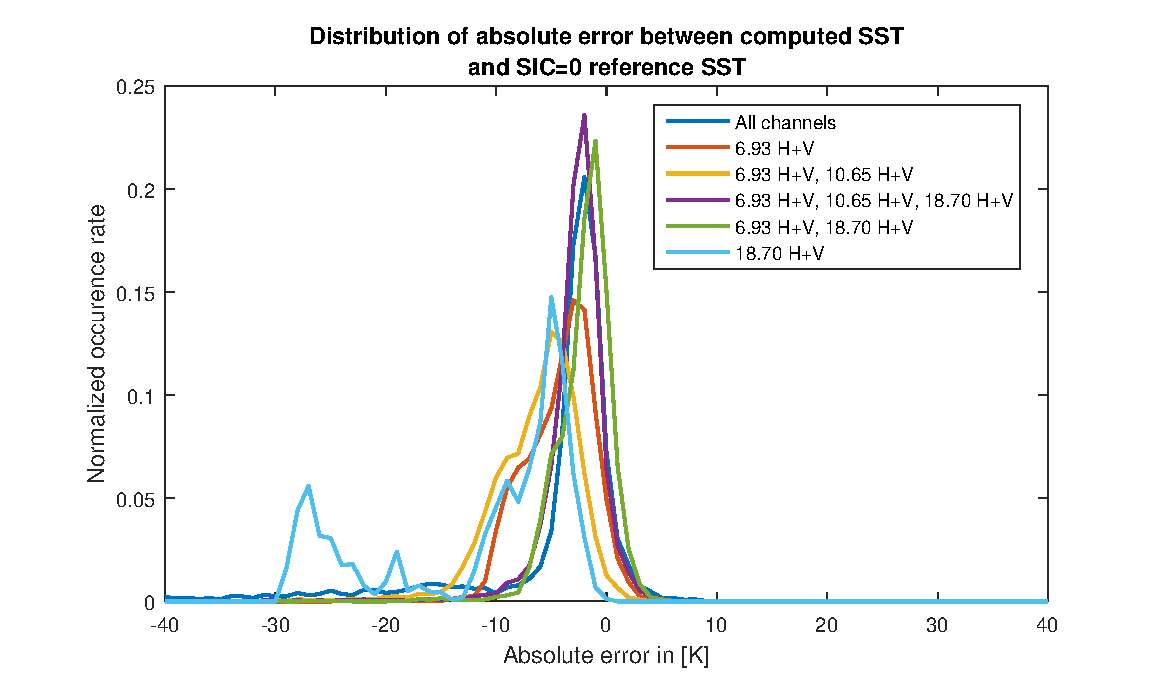
\includegraphics[width=0.9\textwidth]{task3b.eps}
	\caption{Distribution of absolute error between the modelled SST and the SIC0 reference SST for a set of channel selections.}
	\label{fig:task3b}
\end{figure}

The mean and standard deviation of the absolute error between the computed SST for different channel selections and the reference data SST is shown in table \ref{tab:task3b_1}. In table \ref{tab:task3b_1} it can be seen that the inclusion of the 10.65 GHz channel results in a larger deviation from the reference. The optimal channel combination is obtained when combining 6.93 and 18.70 GHz including both polarisations. When evaluating the 6.93 and 18.70 GHz channels individually, the 6.93 GHz channel yields the best result.
\newline 

\begin{table}[h!]
	\centering
	\begin{tabular}{@{}p{9cm}p{3cm}p{3cm}@{}}
		Channel selection [GHz] & Mean [K] & Std. Dev. [K] 
		\tabularnewline
		\midrule
		6.93 H+V, 10.65 H+V, 18.70 H+V, 23.80 H+V, 36.50 H+V & -5.6562 &  18.7487	\\
		6.93 H+V	& -3.7875	&  3.0815 \\
		6.93 H+V, 10.65 H+V	& -6.3362	&  6.5668 \\
		6.93 H+V, 10.65 H+V, 18.70 H+V	& -2.6071 &	5.2244	\\
		6.93 H+V, 18.70 H+V	& -1.5470 & 2.7493	\\
		18.70 H+V	& -10.7803 & 8.8044 \\
		\midrule
	\end{tabular}
	\caption{Mean and standard deviation of the absolute error between the computed SST for different channel selections and the reference data SST.}
	\label{tab:task3b_1}
\end{table}


\subsubsection{Estimated Uncertainties of Inverse Model on SST}
An estimated uncertainty on the SST parameter, as a result of the inversion process, can be determine by computing the S matrix. The S matrix is integrated in the inversion scheme and defined as: 

\begin{equation*}
S =
\Big(S_p^{-1} + M_n^T S_e^{-1} M_n \Big)^{-1}  
\label{S_matrix}
\end{equation*}

If the uncertainties on the starting values for the geophysical parameters in the \(S_p\) matrix are large, it will carry less weight in the iteration and the result of the iteration will be dominated by the measurement error of the radiometer and vice versa. The S matrix is a 7 by 7 matrix in which the diagonal elements are indicative of the inverse model estimated uncertainties on the geophysical parameters, when assuming a perfect forward model. 
\newline

In table \ref{tab:task3b_2} the diagonal element of S corresponding to the SST parameter is listed for each channel selection. The value in the diagonal is a variance and the table \ref{tab:task3b_2} values have been converted to standard deviations by taking the square root of the variance. It is important to note, that the S matrix estimated uncertainties on the SST originates from the inversion and does not take into account any error propagating from the forward model. The S matrix estimated uncertainties is also based on the assumption that the uncertainties \(S_p\) and \(S_e\) are good estimates. 

\begin{table}[h!]
	\centering
	\begin{tabular}{@{}p{11cm}p{4cm}@{}}
		Channel selection & Estimated uncertainties 
		\tabularnewline
		\midrule
		6.93 H+V, 10.65 H+V, 18.70 H+V, 23.80 H+V, 36.50 H+V & 1.2555	\\
		6.93 H+V	& 2.6054	\\
		6.93 H+V, 10.65 H+V	& 2.5347	\\
		6.93 H+V, 10.65 H+V, 18.70 H+V	& 1.4668		\\
		6.93 H+V, 18.70 H+V	& 1.6451	\\
		\midrule
	\end{tabular}
	\caption{Estimated uncertainties when assuming a perfect forward model, computed from S matrix of SST parameter for different channel selections.}
	\label{tab:task3b_2}
\end{table}

The estimated uncertainty is smaller when all channels are used to estimate the SST. Including the 18.70 GHz frequency also improves the inverse model retrieval error on SST.











\subsection{Implementation of the Inverse Model on a Time Series of Open Water Data from the North Atlantic}

The inverse model was applied to a time series of brightness temperatures measured at \SI{45}{\degree}N and \SI{45}{\degree}W (see reference data file, the recalibration was applied). Figure \ref{fig:timeseries} shows the seasonal cycle of the sea surface temperature  as computed by the inverse model. 27 outliers below \SI{270}{K} and three outliers above \SI{300}{K} were removed to keep the scale readable in the relevant area. The plot was smoothed by a moving average filter with a span of \SI{10}{}. The ticks on the horizontal axis denote the start of each month.

\begin{figure}[h]
	\centering
	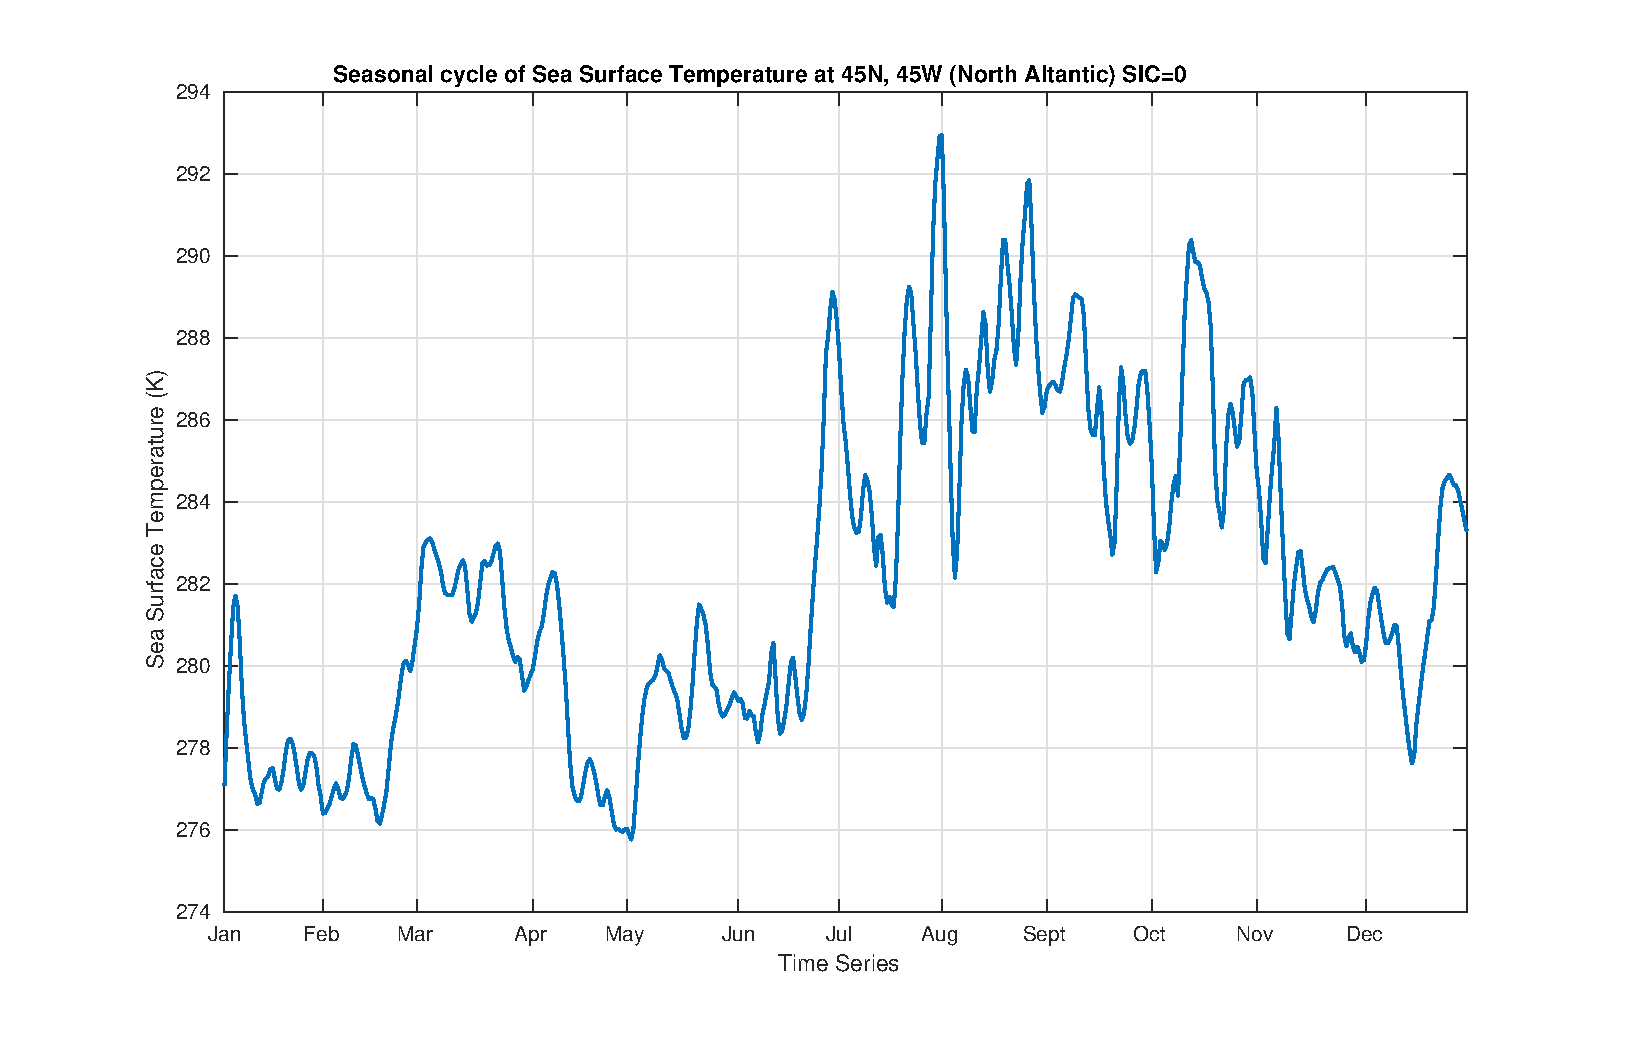
\includegraphics[width=0.9\textwidth]{TimeSeries.eps}
	\caption{Seasonal cycle of the sea surface temperature in the North Atlantic}
	\label{fig:timeseries}
\end{figure}

The sea surface temperature varies over the year, with the temperature for the months August and September ranging up to \SI{293}{K}. For the months January and February, the temperature is generally lower. In this year (2014), the sea surface was warmer in March and April, followed by a lowpoint of approximately \SI{276}{K} in the beginning of May.
\newline

\begin{table}[h]
\centering
\begin{tabular}{@{} l l l l @{}}
 & \multicolumn{3}{c}{Standard Deviation}
\tabularnewline
\cmidrule(l{1mm}){2-4}
 & tcwv [\SI{}{\kilo\gram\per\square\meter}] & tclw [\SI{}{\kilo\gram\per\square\meter}] & ws [\SI{}{m/s}] \\
\midrule
January & \SI{9.0890}{} & \SI{0.1308}{} & \SI{15.6021}{} \\
July & \SI{4.0613}{} & \SI{0.1055}{} & \SI{16.5609}{} \\
\midrule
\end{tabular}
\caption{Standard deviations of water vapor, cloud liquid water and wind speed in winter and summer}
\label{tab:jan_jul}
\end{table}

The standard deviations of water vapor, cloud liquid water and wind speed in January and July were calculated, see Table \ref{tab:jan_jul}. Since the inverse model was found to be less accurate for higher sea surface temparatures, the standard deviation of the parameters measured in the summer may be quite high. It seems, however, that the variability of the wind speed is lower in summer than it is in winter.









\subsection{Exclusion of Ice Parameters in Model Inversion}
The inverse model is applied to the AMSR2 measured brightness temperatures for the dataset with an ice concentration of 0. The inverse model is adjusted such that it disregards the ice temperature, the ice concentration and the multi year ice fraction. The goal is to assess whether the remaining parameters, namely wind speed, water vapour, cloud liquid water and sea surface temperature can be estimated with better accuracy and precision, when the ice parameters are excluded.   

\subsubsection{Exclusion Procedure}
In the first case, no change is made to the inverse model and the ice parameters are included in the inversion process. In the second case the ice parameters are excluded by adjusting the starting values in \(p_0\) and the uncertainties in \(S_p\). The initial guesses for ice temperature, ice concentration and multi-year ice fraction are set to zero in \(p_0\). The diagonal elements of the \(S_p\) matrix corresponding to the ice parameters are set to values near zero, here is used a value of \(10^{-7}\). The diagonal elements in \(S_p\) cannot be exactly zero, as this will prevent the inversion of \(S_p\).  
\newline

The inverse model is applied using the brightness temperatures of the SIC=0 dataset as input. The SIC=0 reference file has 6988 data points, all of which were used. The reduced number of geophysical parameters are computed for the first case where we include the ice parameters in \(p_0\) and for the second case where we exclude the ice paramters in \(p_0\) and adjust \(S_p\). The reference values for the geophysical parameters, \(p_{reference}\), corresponding to the brightness temperatures used as input in the inverse model are subtracted from the computed parameters \(p_{estimate}\) for both cases in the following way:

\begin{equation*}
e = p_\text{estimate} - p_\text{reference}
\end{equation*} 

Distributions of the absolute error are plotted for wind speed, water vapour, cloud liquid water and sea surface temprature in figures \ref{fig:task6_fig_1} to \ref{fig:task6_fig_4}, where the occurence rate has been normalized by the number of data points.   
\newline

\begin{figure}[h]
	\centering
	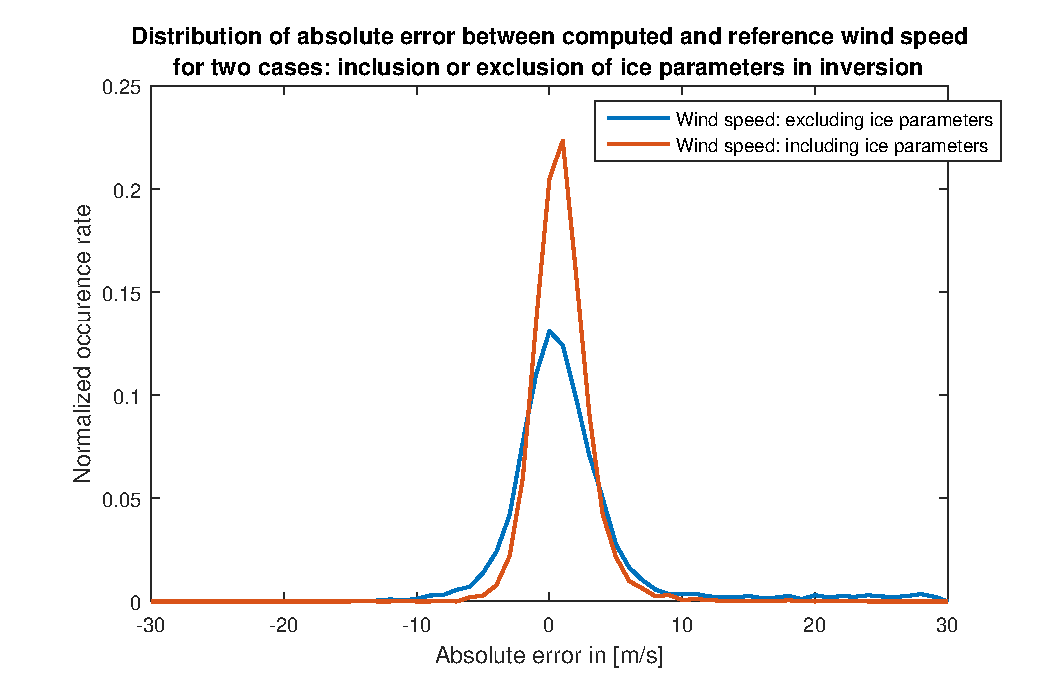
\includegraphics[width=0.9\textwidth]{task6_fig_1.eps}
	\caption{Distribution of absolute error between estimated and the SIC0 reference wind speed for the case where the ice parameters are included in the inversion and for the case where the ice parameters are excluded from the inversion.}
	\label{fig:task6_fig_1}
\end{figure}
\begin{figure}[h]
	\centering
	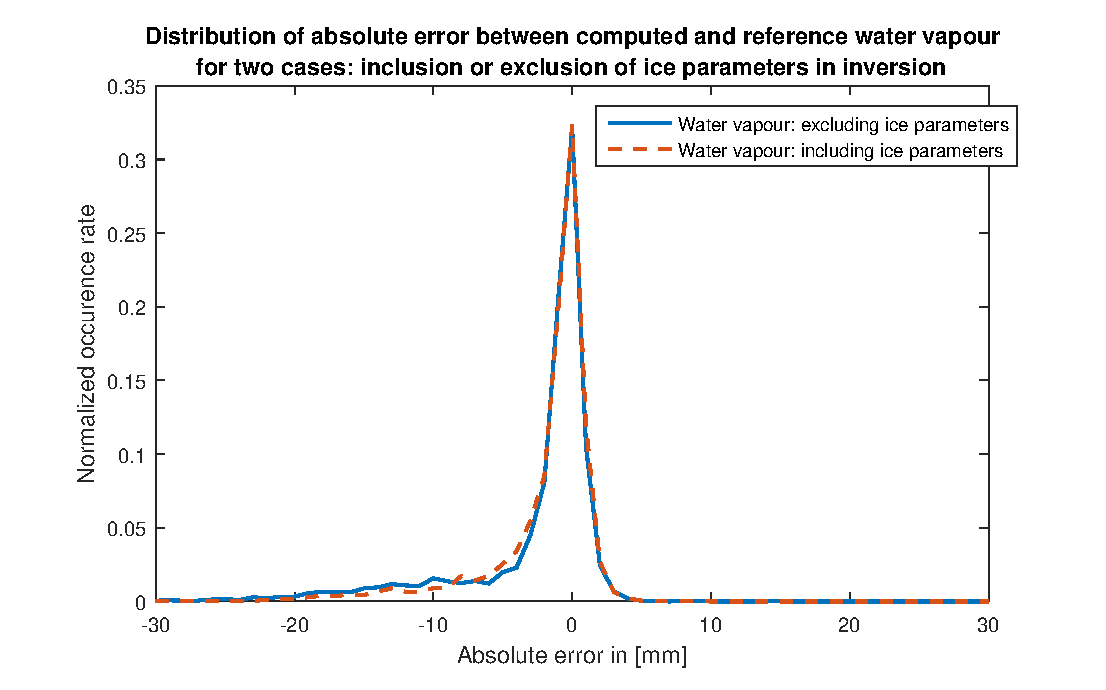
\includegraphics[width=0.9\textwidth]{task6_fig_2.eps}
	\caption{Distribution of absolute error between estimated and the SIC0 reference water vapour for the case where the ice parameters are included in the inversion and for the case where the ice parameters are excluded from the inversion.}
	\label{fig:task6_fig_2}
\end{figure}
\begin{figure}[h]
	\centering
	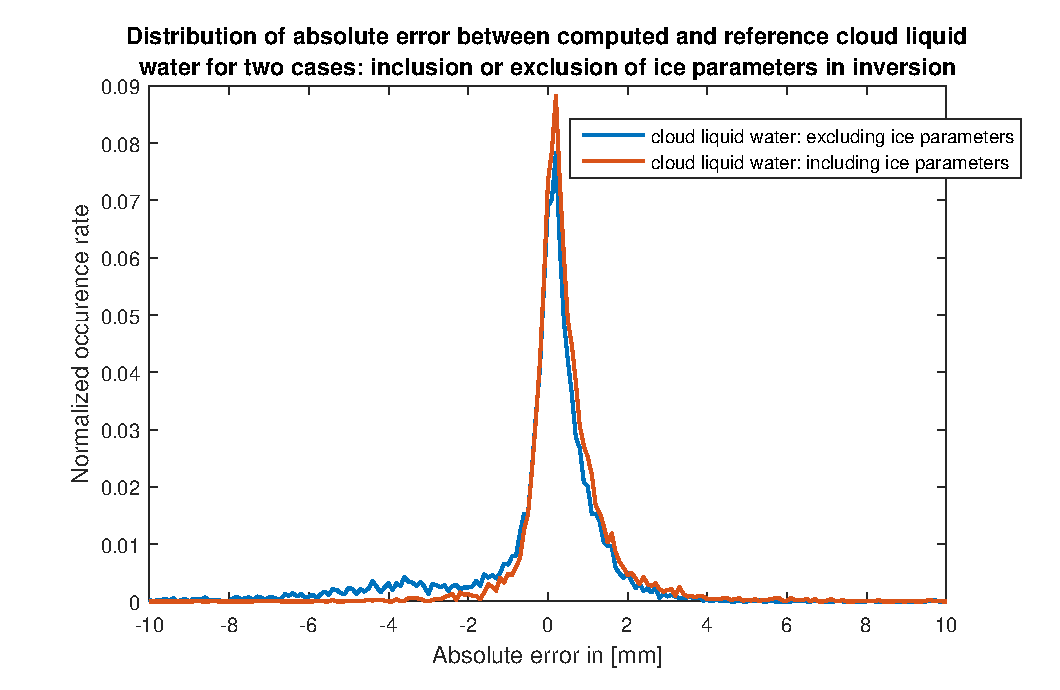
\includegraphics[width=0.9\textwidth]{task6_fig_3.eps}
	\caption{Distribution of absolute error between estimated and the SIC0 reference cloud liquid water for the case where the ice parameters are included in the inversion and for the case where the ice parameters are excluded from the inversion.}
	\label{fig:task6_fig_3}
\end{figure}
\begin{figure}[h]
	\centering
	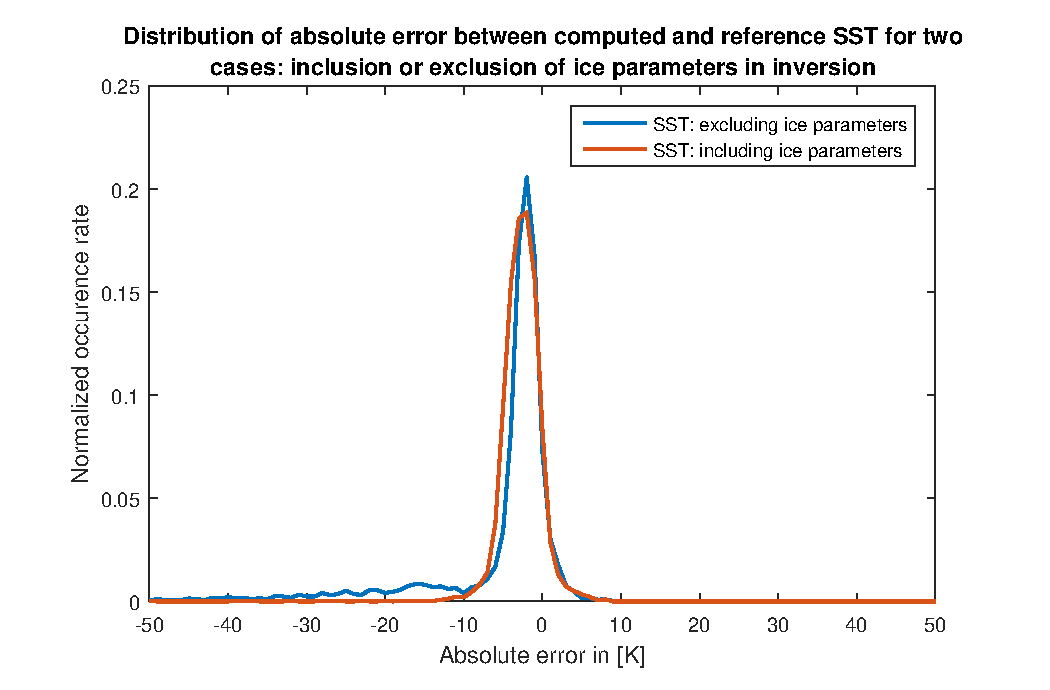
\includegraphics[width=0.9\textwidth]{task6_fig_4.eps}
	\caption{Distribution of absolute error between estimated and the SIC0 reference sea surface temperature for the case where the ice parameters are included in the inversion and for the case where the ice parameters are excluded from the inversion.}
	\label{fig:task6_fig_4}
\end{figure}

The mean and standard deviation of the absolute error between the estimated values and reference values for the two cases are shown in table \ref{tab:task6_tab_1}. In table \ref{tab:task6_tab_1} it can be seen that the precision with which the wind speed, water vapour, cloud liquid water and SST can be retrieved varies greatly from one case to the other. When the ice parameters are excluded, all the remaining parameters can be determined with better precision and arguably also better accuracy. The inverse model is more sensitive to changes in the ice parameters, which causes the model to overshoot in the iteration process. By excluding the ice parameters, the accuracy and precision of the remaining parameters are improved. This is especially the case for wind speed and sea surface temperature. The mean and standard deviation of the ice concentration has been included in table \ref{tab:task6_tab_1} to illustrate the response of the inverse model, when the confidence in the a priori starting guess is high. The degree of freedom of the model is restricted for this case, and the ice parameter output values are forced to approach zero. The change between \(p\) and \(p_{n+1}\) for every iteration normally has large fluctuations, but by restricting the inverse model by predetermining the ice parameters this effect is dampened, and the estimation of the remaining parameters improve.

\begin{table}[h!]
	\centering
	\begin{tabular}{@{}p{4.0cm} p{2.4cm}p{2.4cm}p{2.4cm}p{2.4cm}@{}}
		\tabularnewline
		& \multicolumn{2}{c}{Including ice in inversion} & \multicolumn{2}{c}{Excluding ice from inversion}
		\tabularnewline
		\cmidrule(r{1em}){2-3} \cmidrule(l{1em}){4-5}
		& Mean & Std. Dev. & Mean & Std. Dev.
		\tabularnewline
		\midrule
		Wind speed	& 7.2348 m/s	& 16.2633 m/s		& 1.4218 m/s	& 2.2110 m/s	\\
		Water vapour		& -2.0860 mm	& 5.3944 mm		& -1.4727 mm	& 	4.1543 mm	\\
		Cloud liquid water		& -0.0214 mm	& 0.2105 mm	& 0.0520 mm	& 0.1438 mm	\\
		Sea surface temperature	& -5.6562 K	& 18.7487 K	& -2.1641 K	& 3.0336 K	\\
		Ice concentration  & -0.1395 & 0.4099 & -6.8071$\times10^{-4}$  & 0.0019 \\
		\midrule
	\end{tabular}
	\caption{Mean and standard deviation of the absolute error between estimated and reference values for the case where the ice parameters are included in the inversion and for the case where the ice parameters are excluded from the inversion.}
	\label{tab:task6_tab_1}
\end{table}
 

\subsubsection{Estimated Uncertainties of Inverse Model on Geophysical Parameters}
The estimated uncertainty on the geophysical parameters as a result of the inversion process can be determined by computing the S matrix. In table \ref{tab:task6_tab_1} the diagonal elements of S corresponding to the geophysical parameters have been listed for the case where the ice parameters have been included in the inversion and for the case where the ice parameters have been excluded.
\newline 

\begin{table}[h!]
	\centering
	\begin{tabular}{@{}p{4.0cm}p{3.3cm}p{3.3cm}@{}}
		\tabularnewline
		& \multicolumn{1}{c}{Including ice in inversion} & \multicolumn{1}{c}{Excluding ice from inversion}
		\tabularnewline
		\cmidrule(r{1em}){2-2} \cmidrule(l{1em}){3-3}
		& Retrieval std. dev. & Retrieval std. dev.
		\tabularnewline
		\midrule
		Wind speed	& 1.1715 m/s	& 0.3127 m/s		\\
		Water vapour		& 0.2528 mm	& 0.1997 mm		\\
		Cloud liquid water		& 0.0211 mm	& 0.0101 mm	 \\
		Sea surface temperature	& 1.2555 K	& 0.8971 K 	\\
		\midrule
	\end{tabular}
	\caption{Estimated uncertainties when assuming a perfect forward model, computed from S matrix, of the geophysical parameters for the case where the ice parameters have been included in the inversion and for the case where the ice parameters are excluded.}
	\label{tab:task6_tab_2}
\end{table}

The estimated uncertainties on the geophysical parameters are smaller, when the inverse model is adjusted to disregards the ice parameters.





\begin{comment}
\clearpage
\section{Application of the Inverse Model}

\subsection{Summary: Uncertainties}
\label{sec:uncertainties}

In section \ref{sec:ForValRes}, the discrepancy between the forward model and the reference data was given in terms of brightness temperatures. To gain a better understanding of the significance of a certain error in brightness temperature, the inverse model was applied to compute the error in the geophysical parameters, which corresponds to adding the root mean square error \(\Delta \ T_\text{B}\) of the brightness temperatures given in figure \ref{fig:for0} to the mean value of the brightness temperatures given in the relevant reference data set.

\begin{align*}
& T_\text{B, mean} =  \\
& [ 165.350 \ 84.003 \ 173.818 \ 91.790 \ 195.326 \ 120.459 \ 216.186 \ 159.302 \ 218.686 \ 157.268 ] \\ \\
& \Delta \ T_\text{B} =  \\
& [ 2.378 \ 3.907 \ 5.462 \ 6.899 \ 9.937 \ 12.585 \ 6.556 \ 11.396 \ 6.194 \ 13.484 ] \\ \\
& T_\text{B, mean + rms error} = \\
& [ 167.728 \ 87.910 \ 179.280 \ 98.689 \ 205.263 \ 133.044 \ 222.742 \ 170.698 \ 224.880 \ 170.752]
\end{align*}

\ \\
The atmospheric and oceanic parameters computed for the two brightness temperature vectors above are shown in table \ref{tab:perror}.

\begin{table}[h!]
\centering
\begin{tabular}{@{} l l l l l l l @{}} \tabularnewline
& ws & tcwv & tclw & sst & skt & ci \\
& [\SI{}{m/s}] & [\SI{}{kg\per\square\meter}] & [\SI{}{kg\per\square\meter}] & [\SI{}{K}] & [\SI{}{K}] & [\SI{}{1}] \tabularnewline
\midrule
\(p(T_\text{B, mean})\) & 2.9647 & 18.4426 & 0.1597 & 283.1698 & 269.0328 & 0.0566 \\
\(p(T_\text{B, mean + rms error})\) & 2.3213 & 19.7732 & 0.1675 & 274.4647 & 272.7620 & 0.1215 \\
\(\Delta \ p\) & -0.6434 & 1.3306 & 0.0096 & -8.7051 & 3.7292 & 0.0649
\end{tabular}
\caption{Error in geophysical parameters introduced by the rms error in brightness temperatures}
\label{tab:perror}
\end{table}

The computed difference in geophysical parameters, \(\Delta \ p\), comes itself with the uncertainty of the inverse model, which was described in the previous section. If the forward model was entirely accurate, \(\Delta \ p\) would represent the error of the numerical weather prediction model used in the reference data set. If the numerical weather prediction model was enterily accurate, \(\Delta \ p\) would describe the error of the forward model. In the latter case, however, a large uncertainty would be attached to \(\Delta \ p\), because this error in the forward model would of course influence the computation of \(\Delta \ p\).










\end{comment}



\clearpage
\section{Conclusion}

\begin{itemize}
\item remember people that we used the ``wrong'' correction parameter for the 6.93 channel
\item forward model only working for no ice
\item inverse model only working for not to high sea surface temperatures
\end{itemize}




\clearpage
\begin{thebibliography}{99}

	\bibitem[1]{Dorthe} Dorthe Hofman-Bang, Forward algorithm, September 2003. \newline \url{http://www.seaice.dk/exercises/task3/Matlab/FW_funktion2_is.m} \newline [accessed: 18/11/2017]
	
	%\bibitem[]{IOMASAreport} Dorthe Hofman-Bang and Leif Toudal, Estimating Ice, Ocean and Atmospheric Parameters from Polar Regions from AMSR-E Microwave Radiometer Measurements, Danish Center for Remote Sensing, Technical University of Denmark. 
	
	\bibitem[2]{Wink2} Round Robin Data Package Manual, Version 2.0/, July 2017. Ref: SICCI SIC RRDP-07-17. \newline
	\url{http://www.seaice.dk/undervisning/Sotiris/SICCI_RRDB_Manual_v2.01_20170717.docx} [accessed: 18/11/2017]
	
	\bibitem[3]{remss} (unit conversion) \url{http://www.remss.com/measurements/atmospheric-water-vapor/} [accessed: 18/11/2017]
	
	%\bibitem[4]{Elachi}  C. Elachi, Introduction to the Physics and Techniques of Remote Sensing. John Wiley and Sons, 1987. (section 6.5+7.3)
	%(Hennings reference in his radar altimetry slides for wind speed direction discussion)

	\bibitem[5]{secret} Kyle. A. Hilburn and Chelle L. Gentemann, AMSR2 Calibration: Intercomparison of RSS and JAXA Brightness Temperatures, unpublished.

	
\end{thebibliography}

\end{document}






